\documentclass[12pt]{beamer}

% jezik
\usepackage[serbian]{babel}

% image
\usepackage{float}
\usepackage{graphicx}
\usepackage{tikz}
%\usepackage{animate}
% tema
\setbeamercolor{structure}{fg=beamer@blendedblue}
\definecolor{beamer@blendedblue}{rgb}{0.137,0.466,0.741}
\usecolortheme{whale}
\usefonttheme{professionalfonts}

% teoreme, definicije, napomene i leme
\usepackage{amsthm}

\newtheorem{thm}{Teorema}[section]
\theoremstyle{definition}
\newtheorem{dfn}{Definicija}[section]
\theoremstyle{remark}
\newtheorem{no}{Napomena}[section]
\theoremstyle{plain}
\newtheorem{lem}[thm]{Lema}

% naslov, ime autora i ustanove
\title{Problem izlaska iz \v sume}
\author{Katarina Krivoku\' ca, Dimitrije Gluk\v cevic}
\institute{\small IS Petnica}

% --------------------------------------------------------------------------------

\begin{document}


\begin{frame}
  \titlepage
\end{frame}


\begin{frame}{Originalni problem}
\begin{figure}
\begin{center}
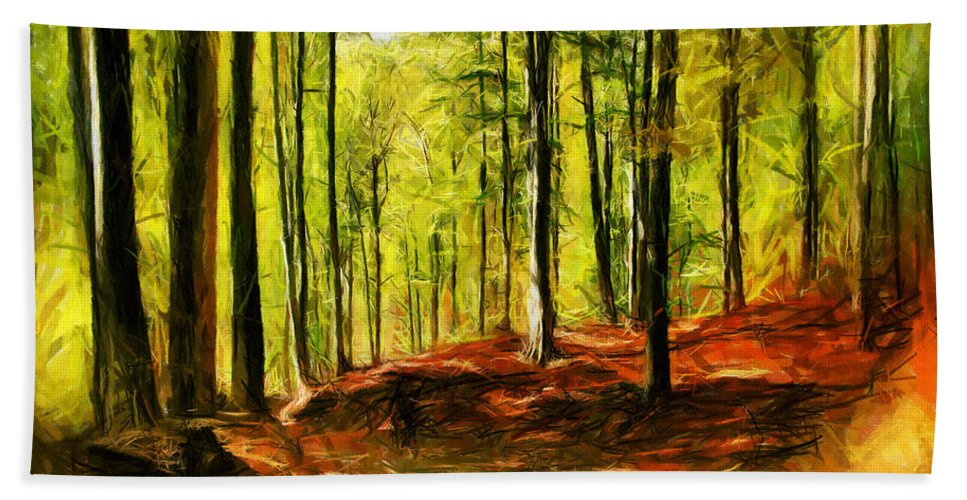
\includegraphics[width=300pt]{suma.jpg}
\end{center}
\end{figure}
\end{frame}




\begin{frame}{\v Sta je poznato?}
\begin{itemize}
\item Problem je re\v sen za vrlo mali broj \v suma
\pause
\item Jedna od tih \v suma je beskona\v cna traka \v sirine 1
\pause
\item Zalgaller je pre skoro 60 godina na\v sao optimalan put za nju
\end{itemize}


%slika Zalgallera

\begin{center}
\begin{tikzpicture}
	\node(img1) {
\includegraphics[width=300pt]{traka.png}};
	\pause
	\node(img) at (-0.2, -0.26) {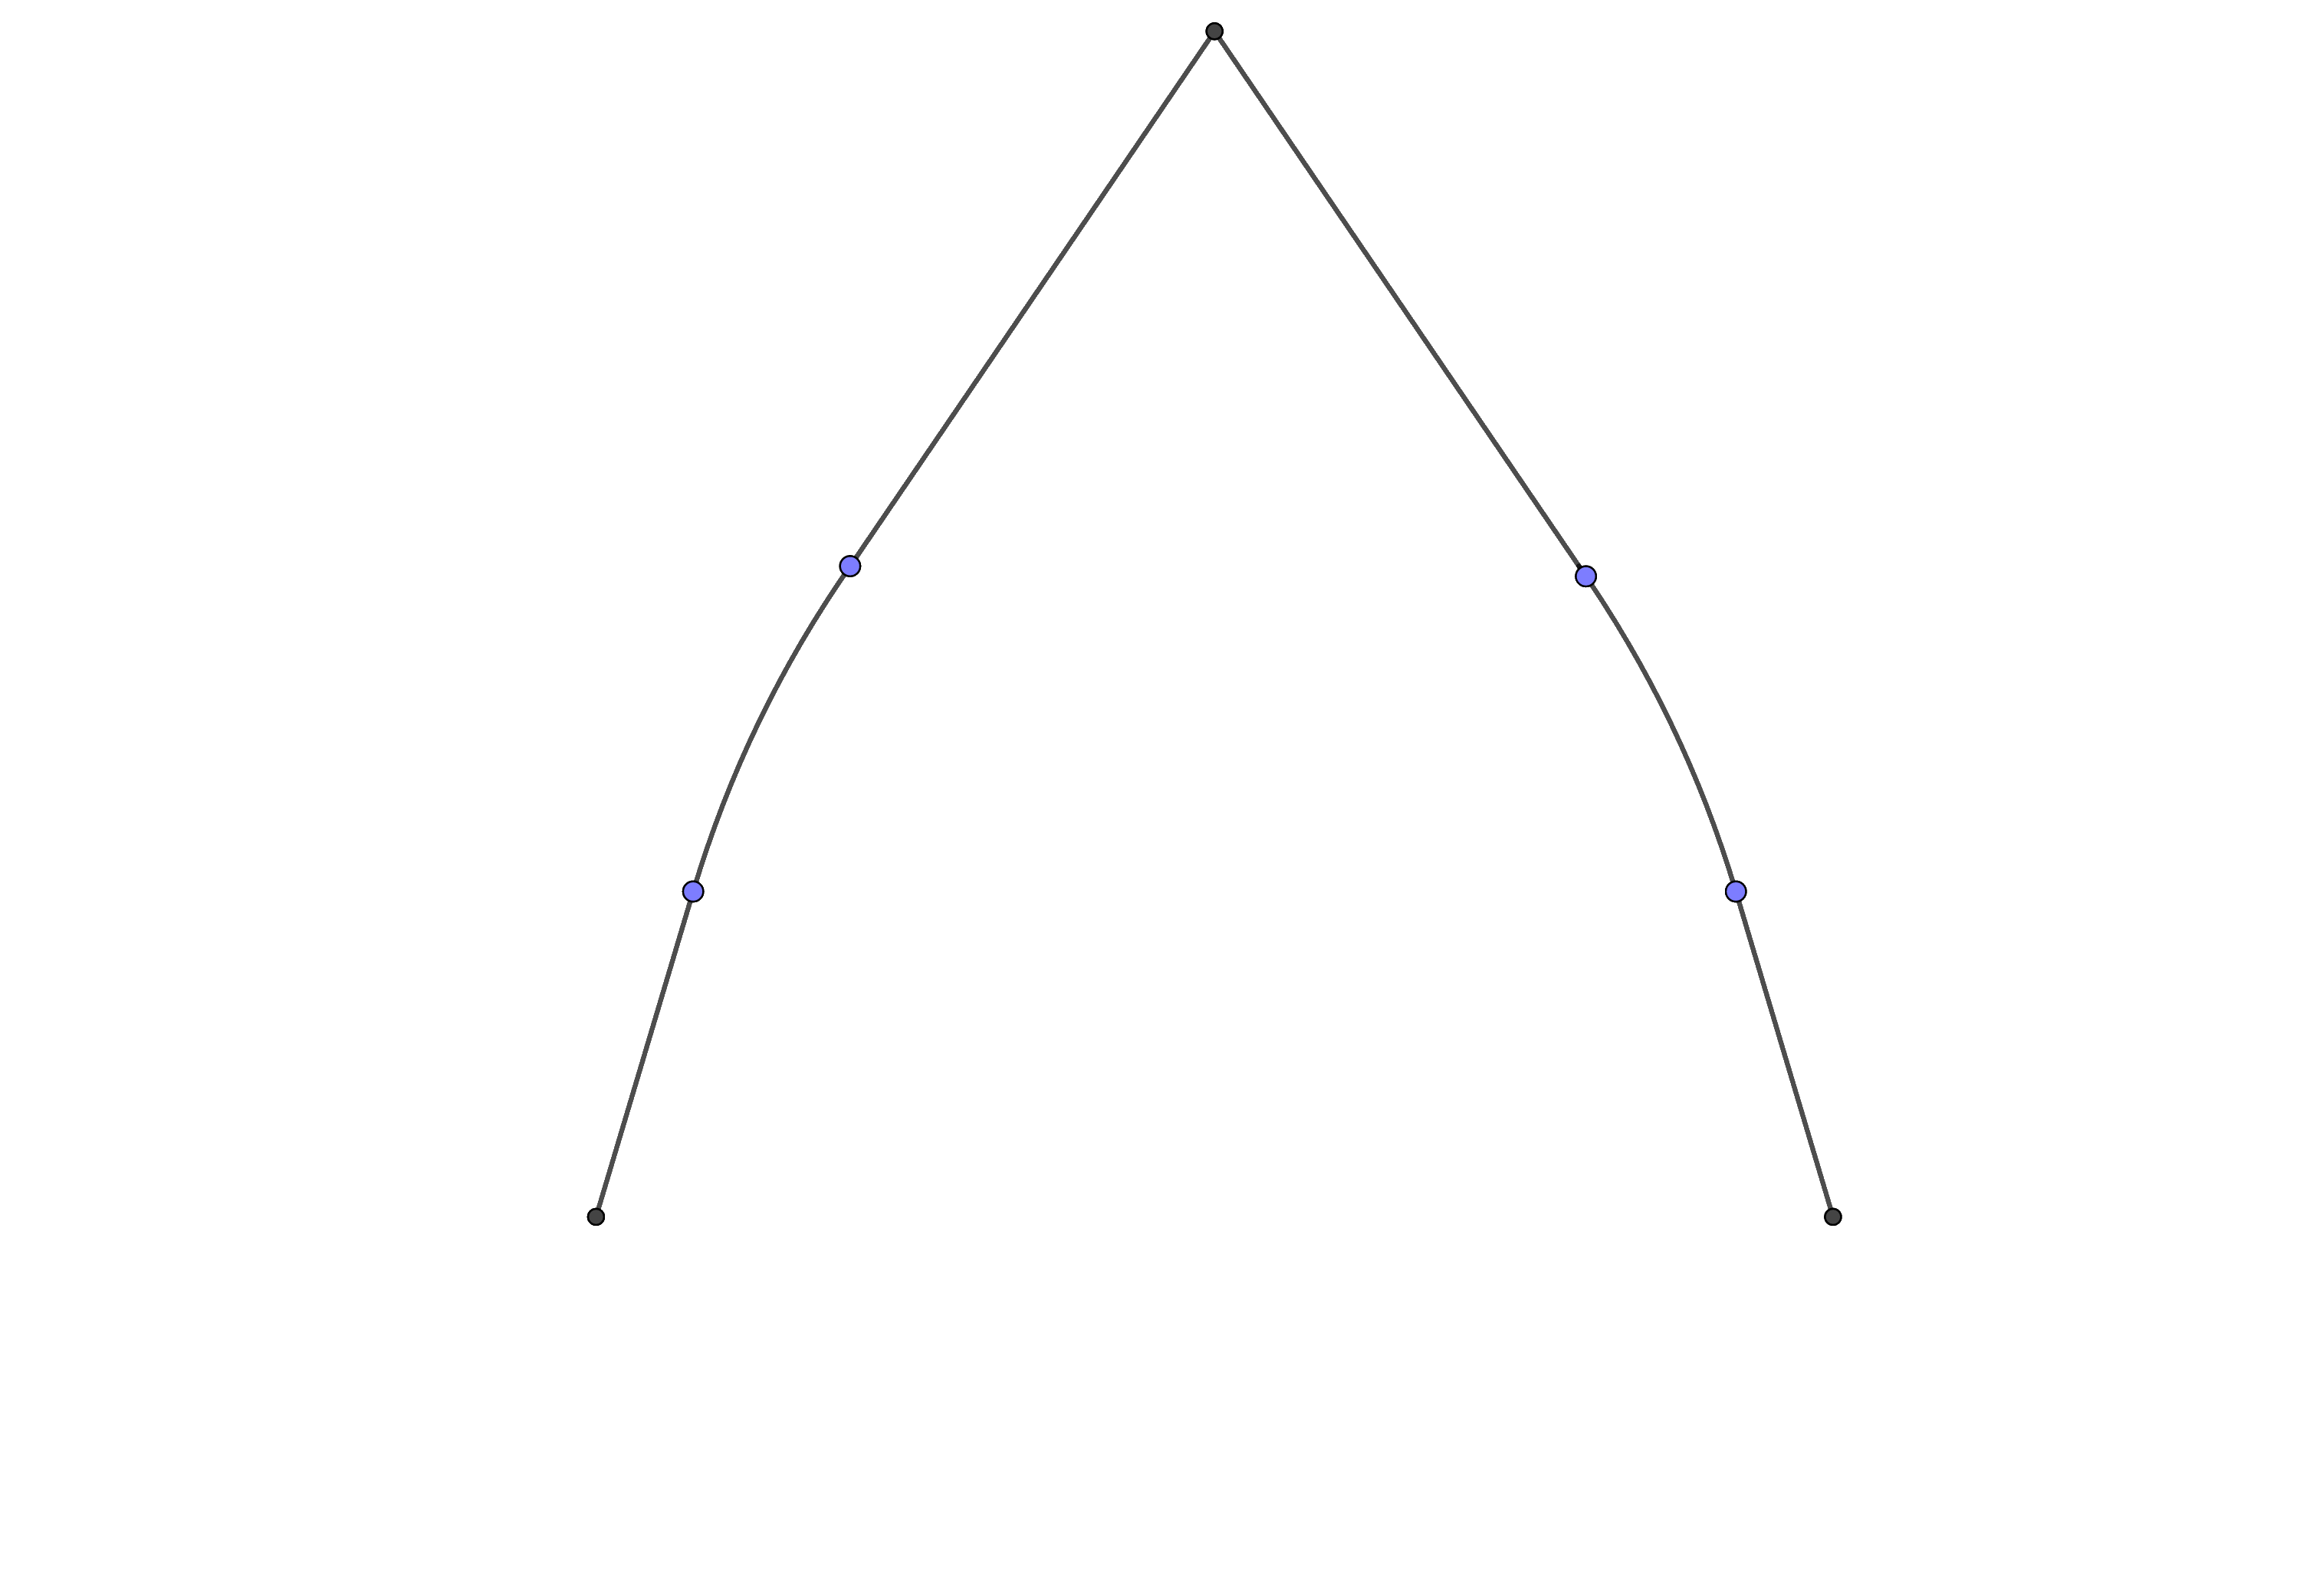
\includegraphics[width=170pt]{zalgaller.png}};
	\pause
\end{tikzpicture}
\end{center}

\end{frame}

\begin{frame}
\begin{itemize}
\item Ovaj problem se i dalje istra\v zuje, ima relativno skoro objavljenih radova
\pause
\begin{figure}
\begin{center}
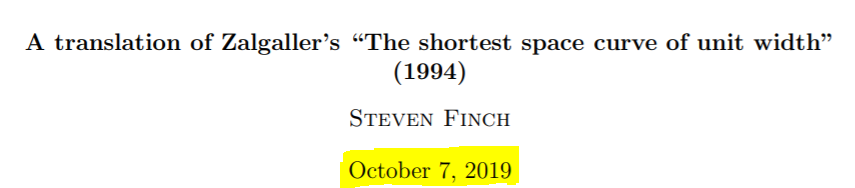
\includegraphics[width=300pt]{6DANA.png}
\end{center}
\end{figure}

\pause
\item A bi\' ce ih i jo\v s...
\pause 
\begin{figure}
\begin{center}
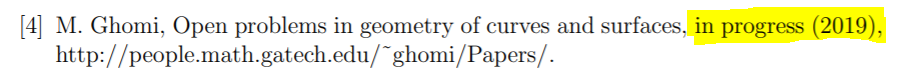
\includegraphics[width=300pt]{progress.png}
\end{center}
\end{figure}

\end{itemize}
\end{frame}

\begin{frame}{Uop\v stenje problema za vi\v se ljudi}
\begin{itemize}
\item A \v sta ako ste u \v sumi sa prijateljima?
\pause 
\begin{figure}
\begin{center}
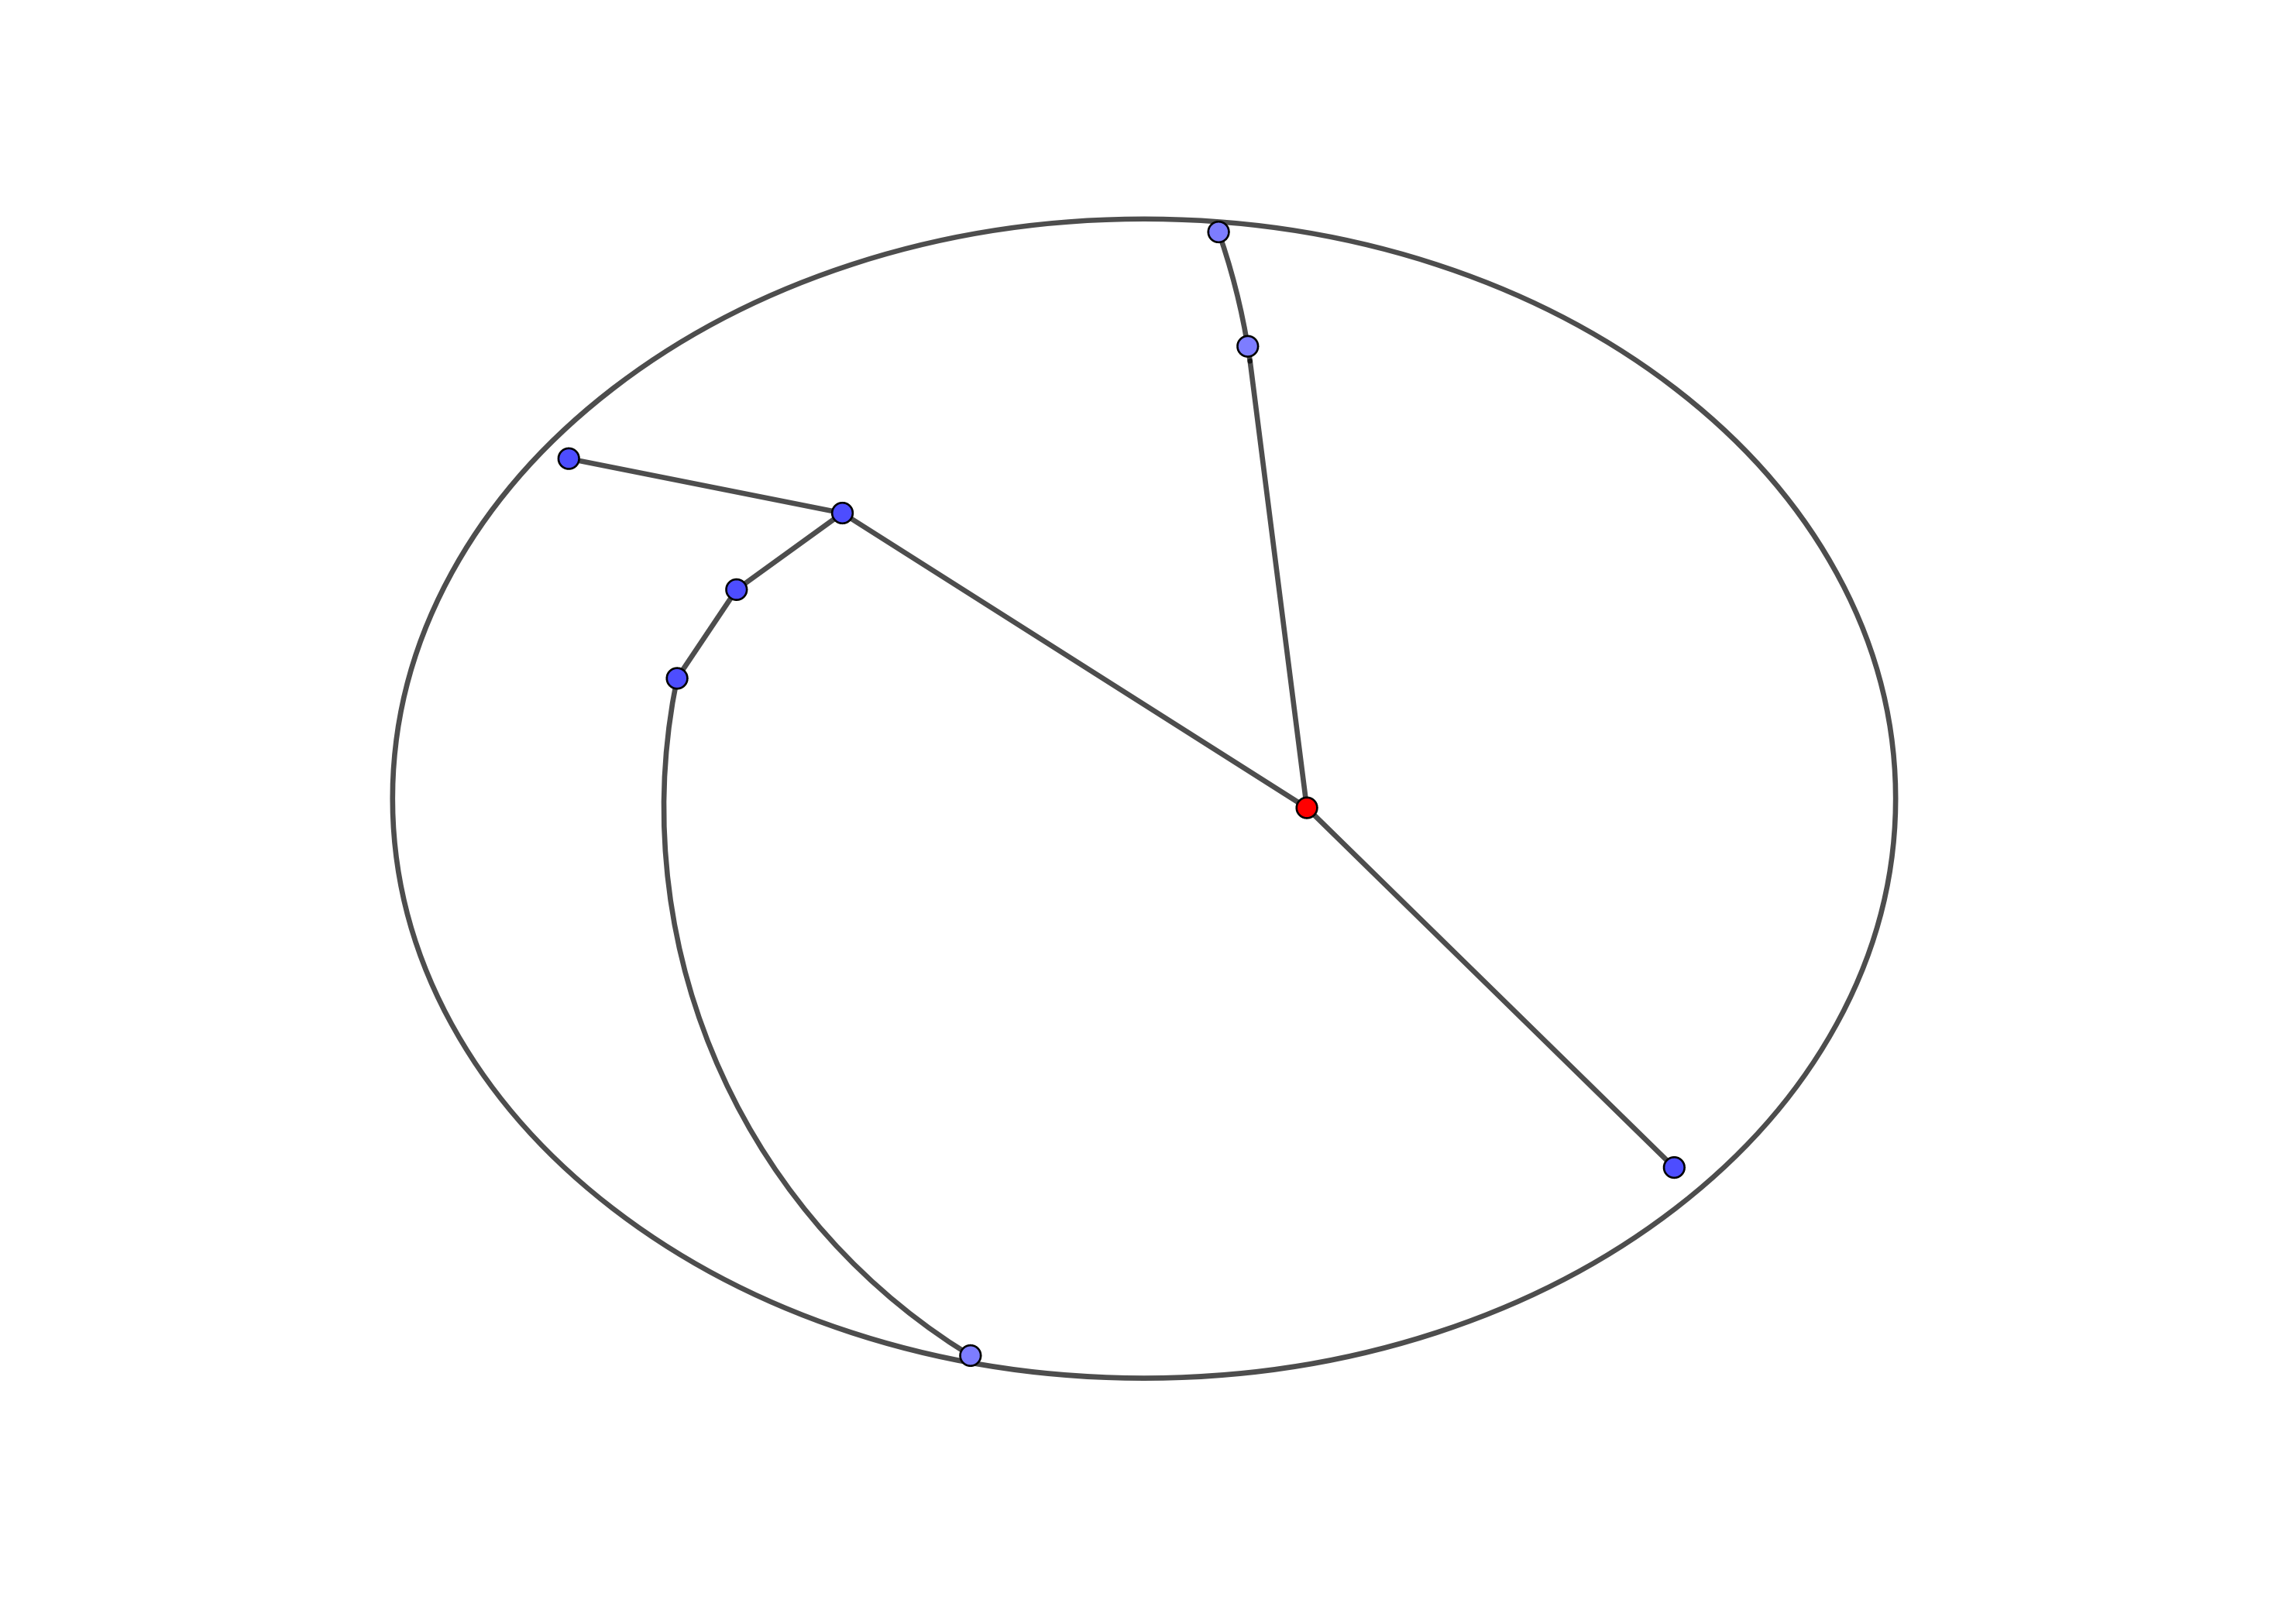
\includegraphics[width=250pt]{vise.png}
\end{center}
\end{figure}

\end{itemize}
\end{frame}

\begin{frame}{Za\v sto je bolje i\' ci sa prijateljima}
\begin{itemize}
\item Dokazano je da je za jednog \v coveka u traci optimalno da se ide Zalgallerovom krivom, koja je du\v zine oko 2.278291644
\pause
\item Sa troje ljudi, iz trake se mo\v ze iza\' ci slede\' cim putem du\v zine 2!
\end{itemize}


\begin{figure}
\begin{center}
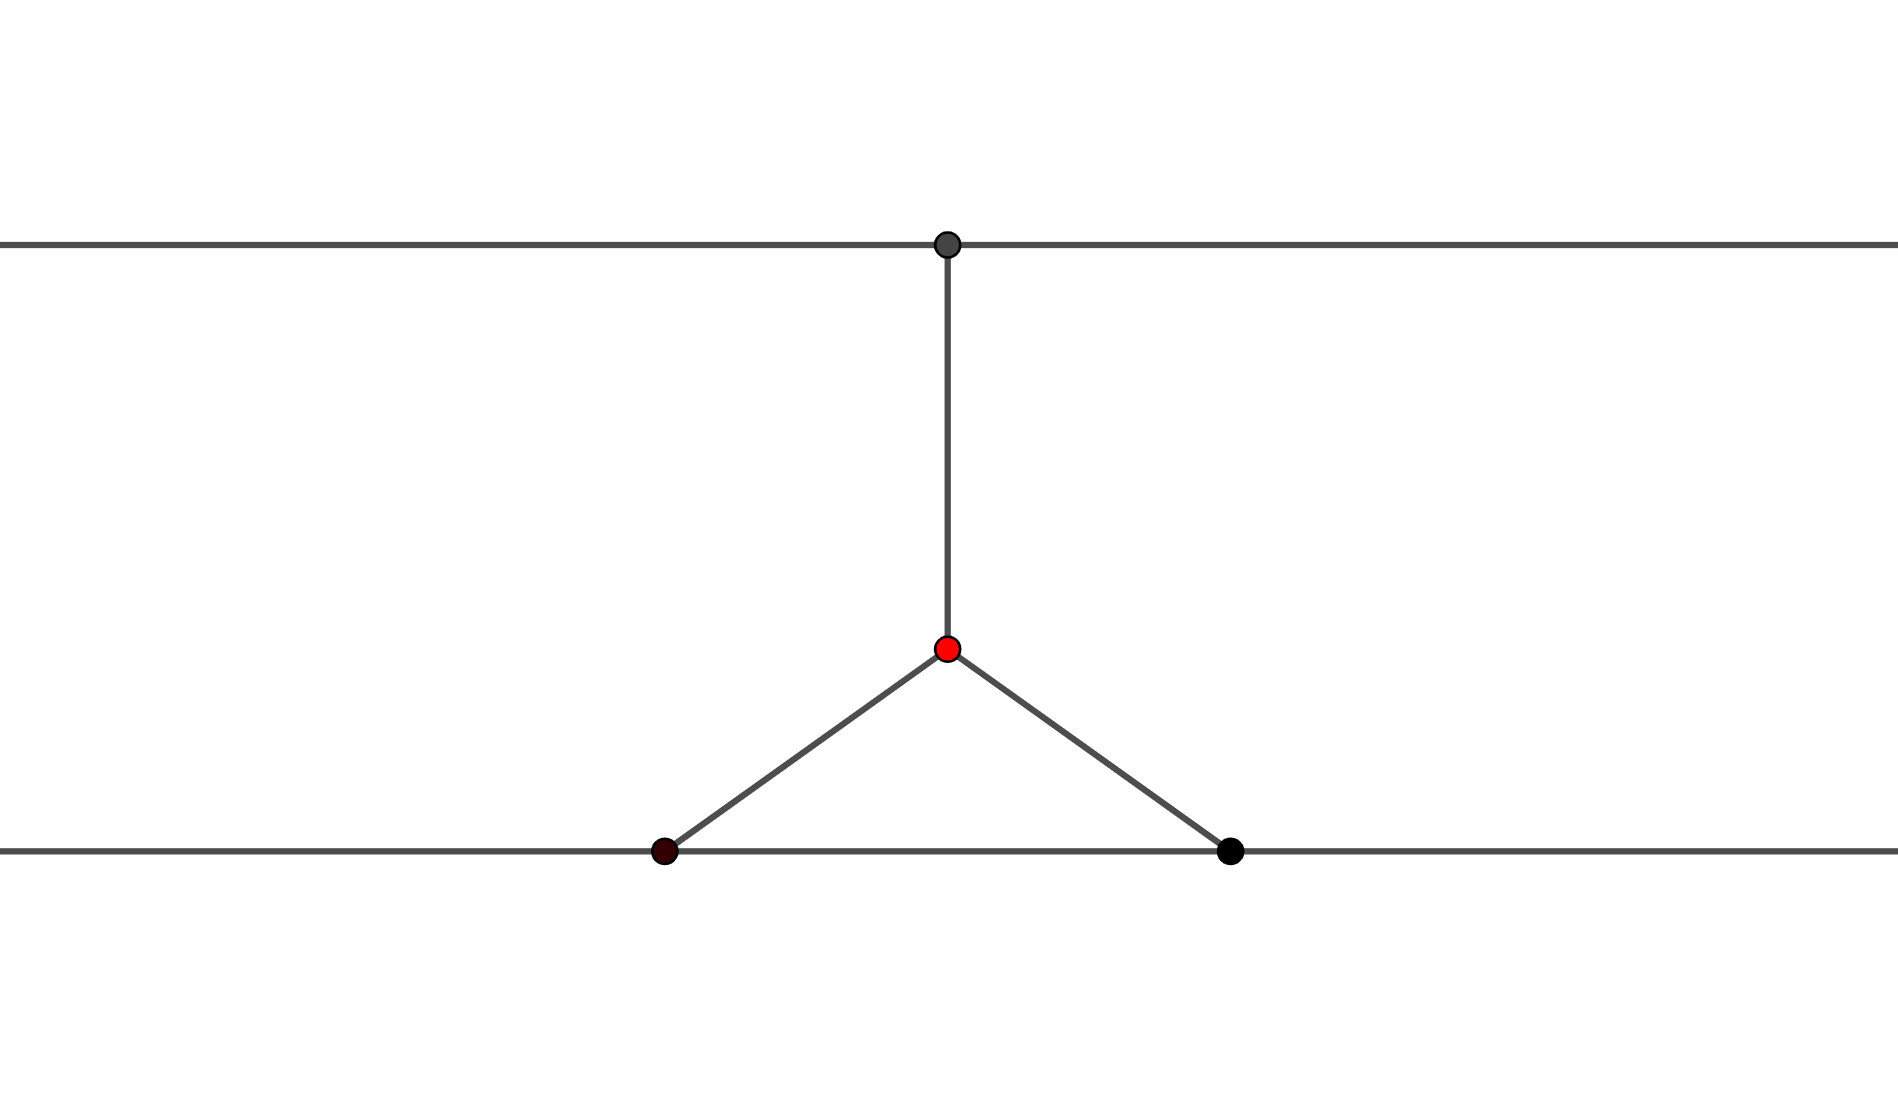
\includegraphics[width=300pt]{trougao.png}
\end{center}
\end{figure}

\end{frame}

\begin{frame}{Rezultati u traci sa vi\v se ljudi}
U \v sumi oblika trake smo posmatrali sve puteve \v ciji je konveksni omota\v c trougao i pokazali smo slede\' ce:
\bigskip
\begin{thm}
U \v sumi oblika trake sa ma koliko ljudi, ne postoji izlazni put kra\' ci od 2 \v ciji je konveksni omota\v c trougao.
\end{thm}
\end{frame}

\begin{frame}{Uop\v stenje problema za vi\v se dimenzija}
\begin{itemize}
\item \v Sumu mo\v zemo sli\v cno definisati i u vi\v sim dimenzijama
\pause
\item U vi\v sim dimenzijama smo posmatrali \v sume sli\v cne beskona\v cnoj traci, koje defini\v semo kao oblast ograni\v cenu sa dve paralelne hiperravni
\end{itemize}
\end{frame}

\begin{frame}{Rezultati u trakama vi\v sih dimenzija}
\begin{itemize}
\item \v Zeleli smo da prona\dj emo neko telo u $n$ dimenzija koje ne mo\v zemo postaviti unutar trake u $n$ dimenzija i prona\dj emo neki put kojim \v covek mo\v ze i\' ci tako da je konveksni omota\v c puta to telo
\pause
\item Telo sa najmanje temena koje ,,\v zivi" u $n$ dimenzijaa je simpleks, mi tra\v zimo najmanji simpleks koji se ne mo\v ze postaviti u ovu \v sumu
\end{itemize}
\end{frame}

\begin{frame}{Rezultati u trakama vi\v sih dimenzija}
\begin{thm}
 Najmanji $n$-simpleks koji se ne mo\v ze postaviti u traku u $n$ dimenzija  je stranice $$\sqrt{\frac{2\left\lceil \frac{n}{2}\right\rceil\cdot \left( n-\left\lceil\frac{n}{2}\right\rceil+1\right)}{n+1}}$$
\end{thm}
%\animategraphics{12}{Rotacija/frame_}{0}{80}
\end{frame}

\begin{frame}{Na\v si rezultati u trakama vi\v sih dimenzija}
\begin{thm}
Postoji izlazan put za jednog \v coveka iz trake u $n$ dimenzija koji je du\v zine $L_{n,1}=n\cdot \sqrt{\frac{2\left\lceil \frac{n}{2}\right\rceil\cdot \left( n-\left\lceil\frac{n}{2}\right\rceil+1\right)}{n+1}}$.
\end{thm}
\begin{figure}
\begin{center}
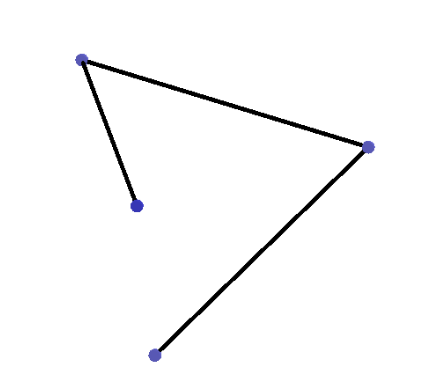
\includegraphics[width=300pt]{jedan.png}
\end{center}
\end{figure}
\end{frame}

\begin{frame}{Rezultati u trakama vi\v sih dimenzija sa vi\v se ljudi}
\begin{thm}
Postoji izlazan put za $n+1$ ljudi iz trake u $n$ dimenzija koji je du\v zine $L_{n,n+1}=\sqrt{n\cdot\left\lceil\frac{n}{2}\right\rceil\cdot\left( n-\left\lceil\frac{n}{2}\right\rceil+1\right)}$.
\end{thm}
\begin{figure}
\begin{center}
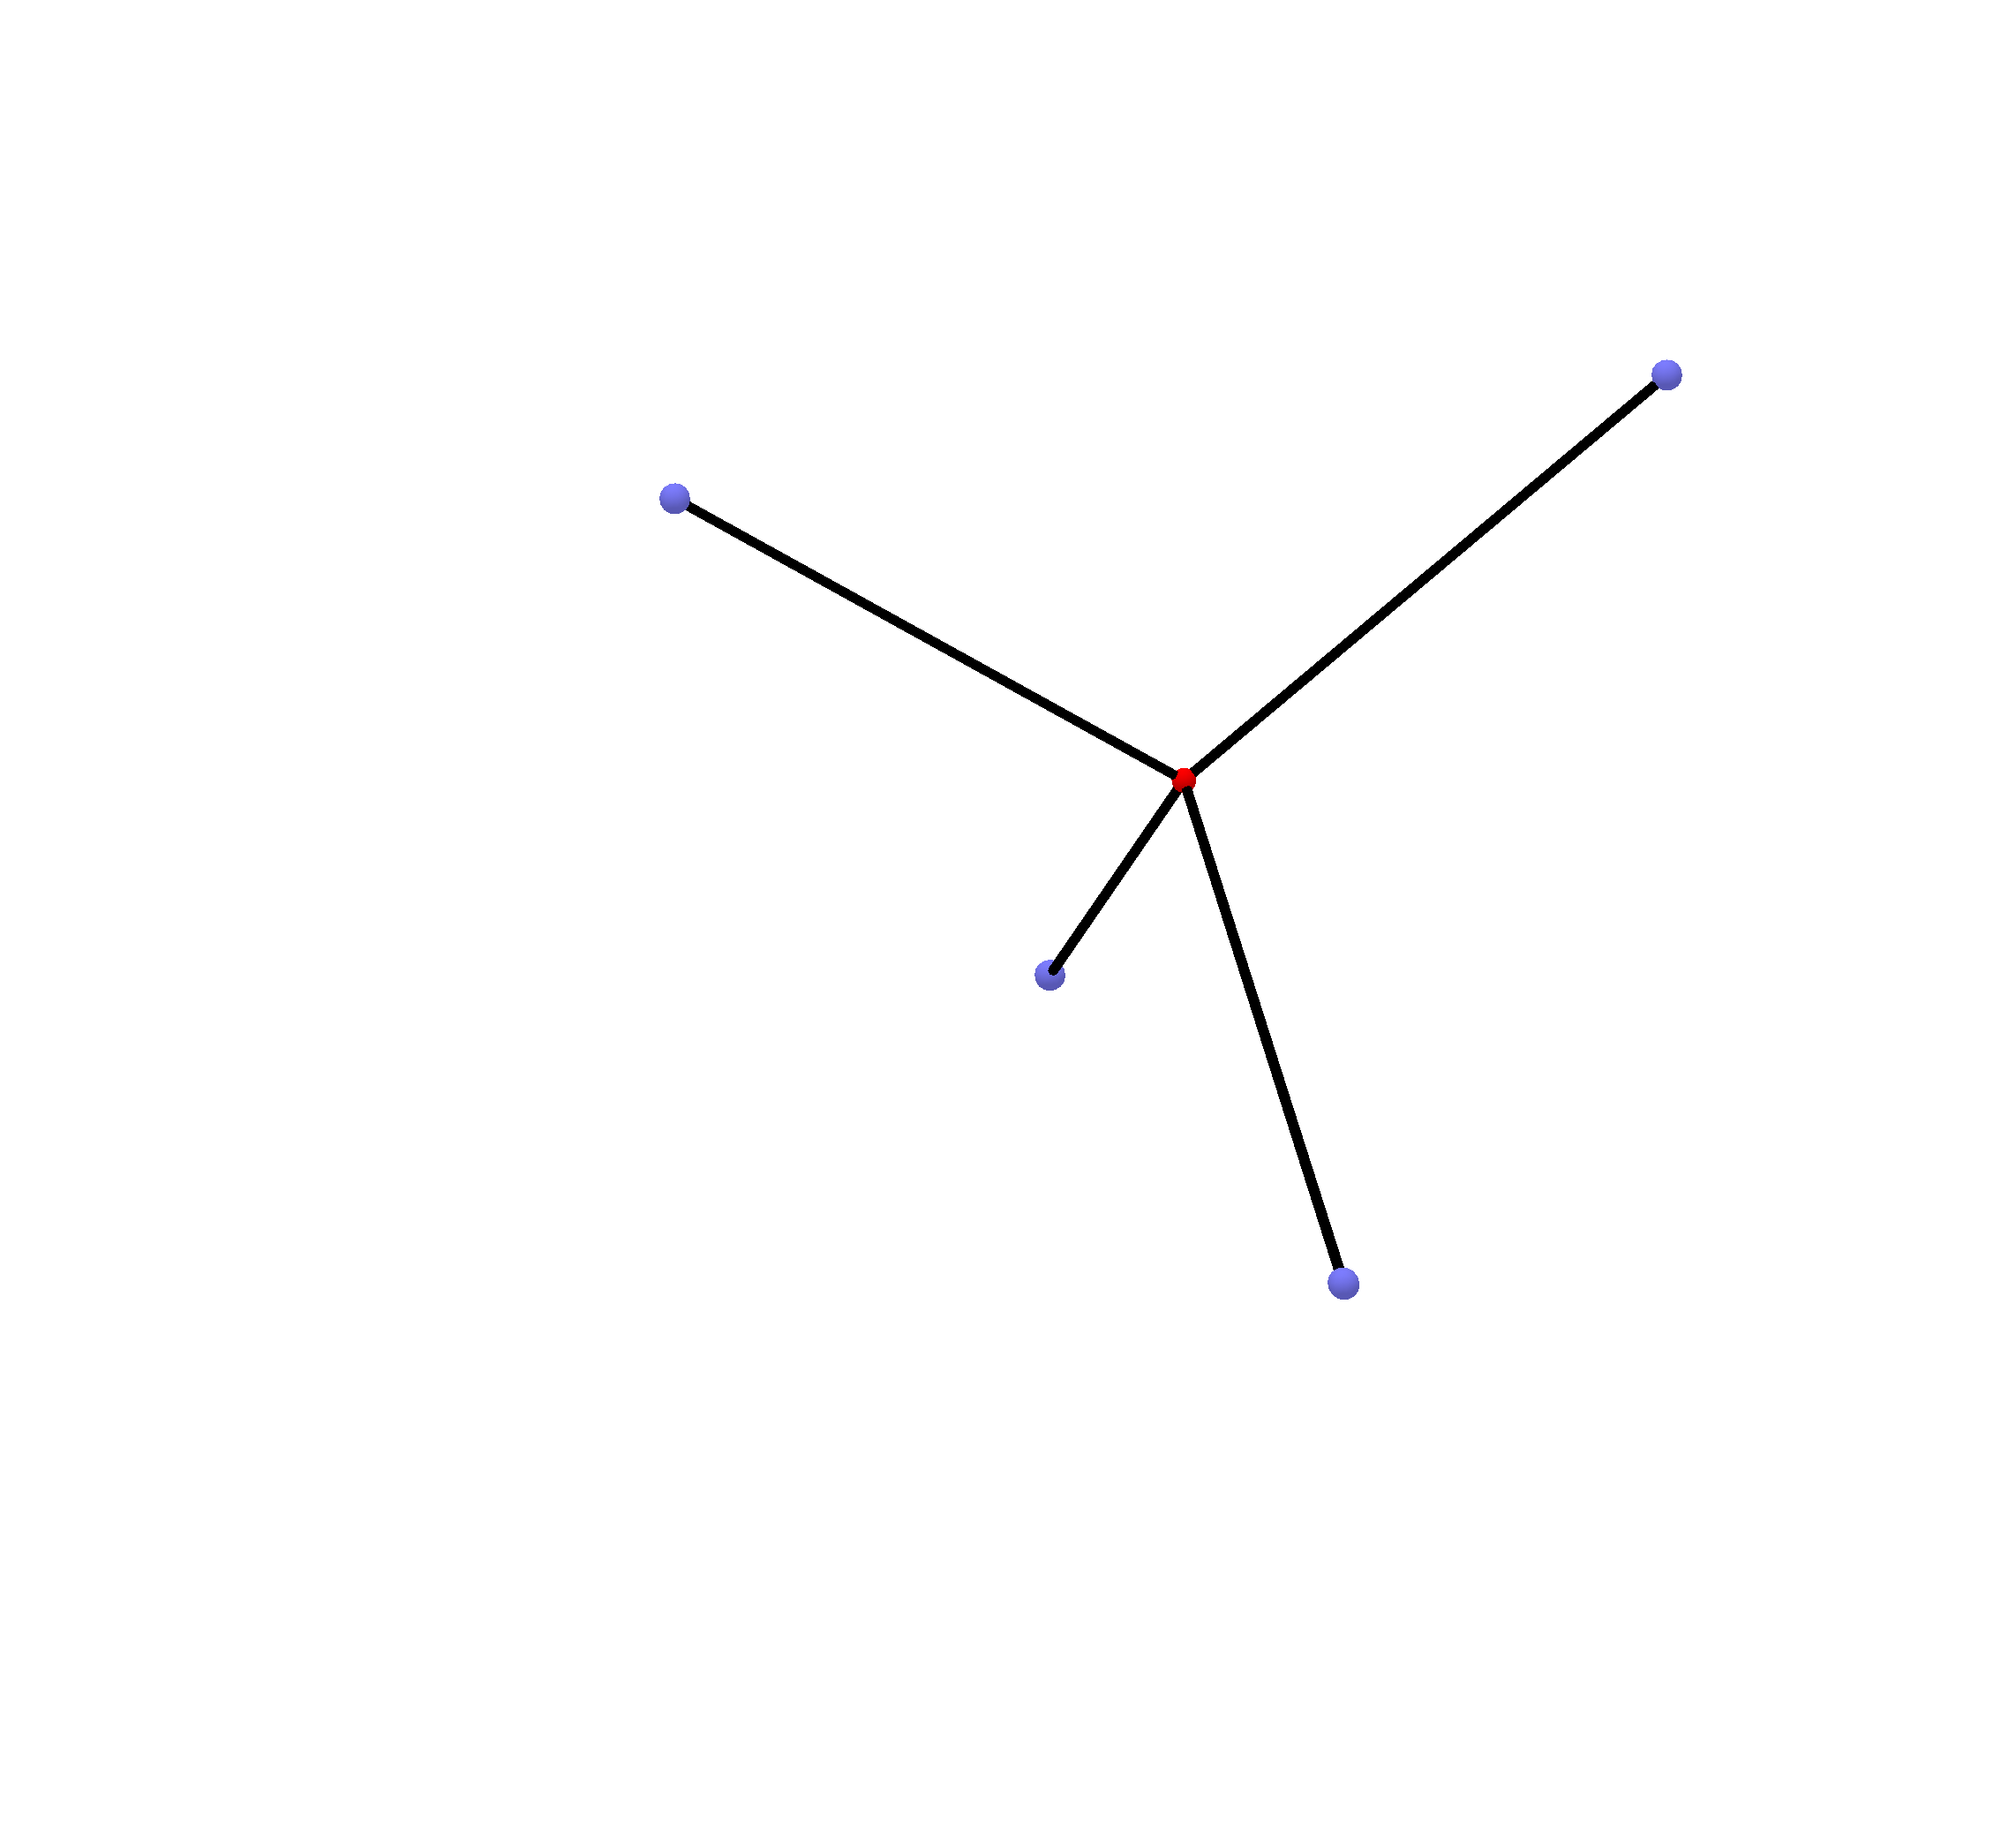
\includegraphics[width=300pt]{cetiri.png}
\end{center}
\end{figure}
\end{frame}

\begin{frame}{Jo\v s neke \v sume u vi\v se dimenzija koje smo posmatrali}
\begin{itemize}
\item Traku iz originalnog problema smo mogli druga\v cije uopstiti
\pause
\item Drugo uop\v stenje koje smo posmatrali je da \v suma koja "\v zivi" u $n$ dimenzija bude ograni\v cena svim ta\v ckama na jednakoj udaljenosti od nekog $k$ potprostora, tu \v sumu nazovimo $k$-trakom u $n$ dimenzija
\pause
\item Primer za to bi bio beskona\v cni valjak u tri dimenzije 
\end{itemize}
\end{frame}

\begin{frame}{Rezultati u tim \v sumama}
\v Zeleli smo ovaj problem da svedemo na neki koji smo ve\' c re\v sili i ispostavilo se da su slede\' ci problemi ekvivalentni
\bigskip
\begin{thm}
Najkra\' ca izlazna putanja iz $k$-trake u $n$ dimenzija je ista kao najkra\' ca izlazna putanja iz trake u $k+1$ dimenzija i obratno.
\end{thm}
\end{frame}

\begin{frame}
\huge {Hvala na pa\v znji!}
\end{frame}

%%%%%%%%%%%%%%%55
\end{document}
